% What quantum mechanics changes for communication (notebook 52, Figure 1).
% (a) Alice sends a qubit through a quantum channel; Eve couples a probe to it with a unitary U. She cannot keep a
%     copy (no-cloning, Section 4), and if the signal states are nonorthogonal, every bit of information she gains
%     shows up as errors at Bob (information gain implies disturbance, Section 5).
% (b) Any physical channel is a unitary coupling to an environment that is then discarded; the result is the Kraus
%     form E(rho) = sum_k K_k rho K_k^dagger with sum_k K_k^dagger K_k = 1 (Section 8). The environment is where
%     the lost information goes, and in cryptography it is assumed to be held by Eve.
\documentclass[tikz,border=6pt]{standalone}
\usepackage{amsmath,amssymb,dsfont}
\usetikzlibrary{arrows.meta,positioning,calc}
\begin{document}
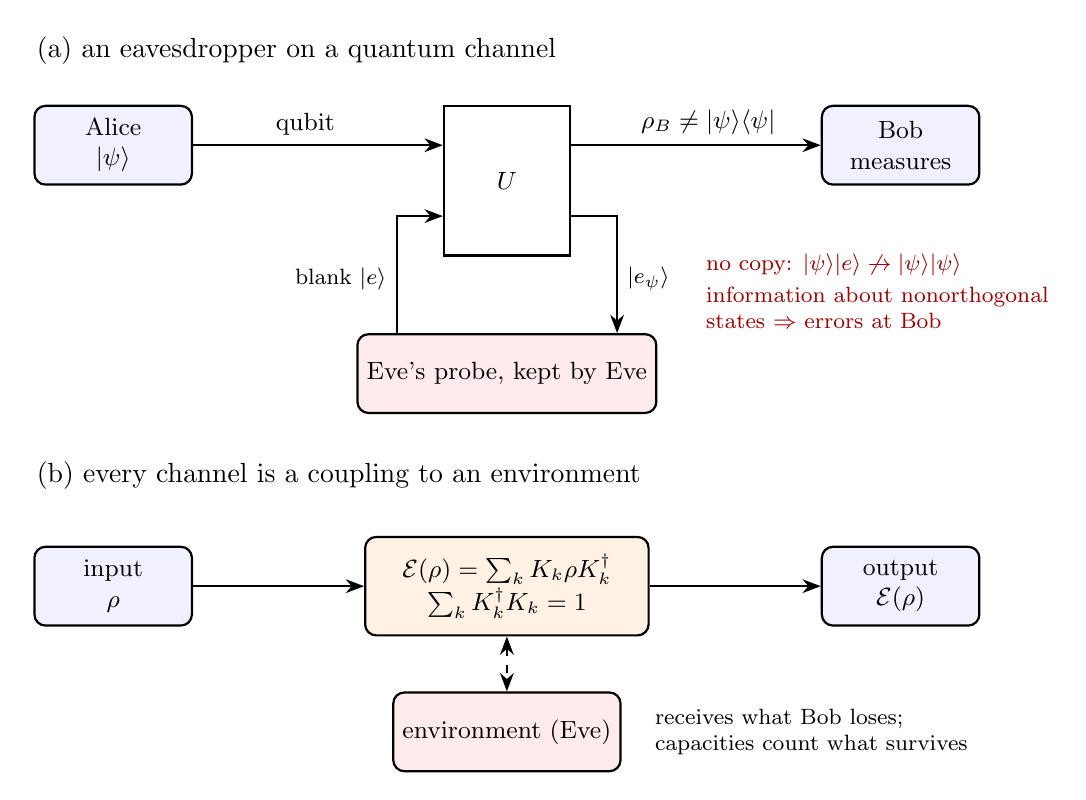
\begin{tikzpicture}[thick, >=Stealth, font=\small,
    party/.style={draw, rounded corners, fill=blue!6, minimum width=2.0cm, minimum height=1.0cm, align=center},
    adv/.style={draw, rounded corners, fill=red!8, minimum width=2.0cm, minimum height=1.0cm, align=center},
    gate/.style={draw, fill=white, minimum width=1.6cm, minimum height=1.9cm},
    chan/.style={draw, rounded corners, fill=orange!10, minimum width=3.6cm, minimum height=1.25cm, align=center}]
  % ---------------- (a) eavesdropping on a quantum channel ----------------
  \node[font=\normalsize, anchor=west] at (-1.1,1.2) {(a) an eavesdropper on a quantum channel};
  \node[party] (A) at (0,0) {Alice\\ $\vert\psi\rangle$};
  \node[party] (B) at (10,0) {Bob\\ measures};
  \node[gate] (U) at (5,-0.45) {$U$};
  \draw[->] (A) -- (U.west |- A) node[pos=0.45, above] {qubit};
  \draw[->] (U.east |- A) -- (B) node[pos=0.55, above] {$\rho_B\neq\vert\psi\rangle\langle\psi\vert$};
  \node[adv, minimum width=3.4cm] (E) at (5,-2.9) {Eve's probe, kept by Eve};
  \draw[->] (3.6,-2.9 |- E.north) -- (3.6,-0.9) -- (U.west |- 0,-0.9);
  \node[font=\footnotesize, left] at (3.6,-1.7) {blank $\vert e\rangle$};
  \draw[->] (U.east |- 0,-0.9) -- (6.4,-0.9) -- (6.4,-2.9 |- E.north);
  \node[font=\footnotesize, right] at (6.4,-1.7) {$\vert e_\psi\rangle$};
  \node[font=\footnotesize, align=left, anchor=north west, text=red!60!black] at (7.4,-1.25)
       {no copy: $\vert\psi\rangle\vert e\rangle\not\to\vert\psi\rangle\vert\psi\rangle$\\[2pt]
        information about nonorthogonal\\ states $\Rightarrow$ errors at Bob};
  % ---------------- (b) a channel is a coupling to an environment ----------------
  \begin{scope}[shift={(0,-5.6)}]
    \node[font=\normalsize, anchor=west] at (-1.1,1.4) {(b) every channel is a coupling to an environment};
    \node[party] (A2) at (0,0) {input\\ $\rho$};
    \node[chan] (C) at (5,0) {$\mathcal E(\rho)=\sum_k K_k\rho K_k^\dagger$\\ $\sum_k K_k^\dagger K_k=\mathds 1$};
    \node[party] (B2) at (10,0) {output\\ $\mathcal E(\rho)$};
    \draw[->] (A2) -- (C);
    \draw[->] (C) -- (B2);
    \node[adv] (Env) at (5,-1.85) {environment (Eve)};
    \draw[<->, dashed] (C.south) -- (Env.north);
    \node[font=\footnotesize, align=left, anchor=west] at (6.75,-1.85)
         {receives what Bob loses;\\ capacities count what survives};
  \end{scope}
\end{tikzpicture}
\end{document}
